
\documentclass{article}
\usepackage[utf8]{inputenc}

\title{Markov Chains, Random Walks, and PageRank}
\author{Jackson Ellinger and Jack Wei}
\date{December 3, 2021}
\usepackage{listings,xcolor,lstautogobble}
\setlength{\oddsidemargin}{0px}
\setlength{\textwidth}{460px}
\setlength{\voffset}{-1.5cm}
\setlength{\textheight}{20cm}
\setlength{\parindent}{0px}
\setlength{\parskip}{10pt}
\usepackage{graphicx}

%% Adapted from 15150 Homework LaTeX Template
% code style
\definecolor{background_color}{RGB}{255, 255, 255}
\definecolor{string_color}    {RGB}{255, 0,   255}
\definecolor{identifier_color}{RGB}{  0,   0,   0}
\definecolor{keyword_color}   {RGB}{ 64, 100, 255}
\definecolor{comment_color}   {RGB}{  34, 139, 34}
\definecolor{number_color}    {RGB}{ 84,  84,  84}
\lstdefinestyle{21241code}{
	basicstyle=\ttfamily,
	numberstyle=\tiny\ttfamily\color{number_color},
	backgroundcolor=\color{background_color},
	stringstyle=\color{string_color},
	identifierstyle=\color{identifier_color},
	keywordstyle=\color{keyword_color},
	commentstyle=\color{comment_color},
	numbers=left,
	frame=none,
	columns=fixed,
	tabsize=4,
	breaklines=true,
	keepspaces=true,
	showstringspaces=false,
	captionpos=b,
	autogobble=true,
	mathescape=true,
}
\lstdefinelanguage{julia}
{
	sensitive=true,
	alsoother={\$},
	morecomment=[l]\#,
	morecomment=[n]{\#=}{=\#},
	morestring=[s]{"}{"},
	morestring=[m]{'}{'},
	morekeywords={
		exit,whos,edit,load,is,
		isa,isequal,typeof,tuple,ntuple,
		uid,hash,finalizer,convert,promote,
		subtype,typemin,typemax,realmin,realmax,
		sizeof,eps,promote_type,method_exists,applicable,
		invoke,dlopen,dlsym,system,error,
		throw,assert,new,Inf,Nan,
		pi,im,begin,while,for,
		in,return,break,continue,macro,
		quote,let,if,elseif,else,
		try,catch,end,bitstype,ccall,
		do,using,module,import,export,
		importall,baremodule,immutable,local,global,
		const,Bool,Int,Int8,Int16,
		Int32,Int64,Uint,Uint8,Uint16,
		Uint32,Uint64,Float32,Float64,Complex64,
		Complex128,Any,Nothing,None,function,
		type,typealias,abstract
	},
}

% code inline
\newcommand{\code}[2][]{{\sloppy
		\ifmmode
		\text{\lstinline[language=julia,style=21241code,#1]`#2`}
		\else
		{\lstinline[language=julia,style=21241code,#1]`#2`}%
		\fi}}

% code block
\lstnewenvironment{codeblock}[1][]{\lstset{language=julia,style=21241code,#1}}{}

% code imported from a file
\newcommand{\codefile}[2][]{\lstinputlisting[language=julia,style=21241code,frame=single,#1]{#2}}
\begin{document}


\maketitle


\section{Mathematical Background}
PageRank is an algorithm developed to rank website pages based on how different pages are connected to each other. To understand how this works, you need to understand how Markov matrices work, what eigenvectors and eigenvalues are and how to find them, how to perform a random walk on a Markov matrix, and what to do if the matrix you make given the web is not a Markov matrix. 

First, a $n$ x $n$ matrix $M$ is a Markov matrix if $M_{ij} \geq 0$ for $1 \leq i, j \leq n$. This means that it has non-negative entries. Additionally, $\sum_{i = 1}^{n} M_{ij} = 1$ for $1 \leq j \leq n$. This means that the column sum is equal to 1. For PageRank, we can apply this idea to our situation of trying to develop PageRank by creating a Markov matrix where the columns correspond with the departing page and the rows correspond with the page where a user would arrive. For example, if you look at the entry in column 1 and row 1, that will correspond with the probability of going from the page that corresponds with column 1 to the page that corresponds with row 1. To calculate the probability of going from the departing page to the page you arrive, you need to look at the total number of pages you could go to from the departing page and assume there is an equal probability to go to any of them. So for example, consider thinking of a set of linked pages as a web. Consider 3 pages named A, B, and C. Say for example that A is linked to B and C. We can then conclude that there is a 1/2 probability of going from the departing page, A, to B, and a 1/2 probability of going from the departing page, A, to C. Since probability will add up to 1, if we translate this into a matrix, the sum of the entries of the columns will equal 1, fulfilling a characteristic of the Markov matrix. Additionally, probability is always non-negative, so all the entries will be greater than or equal to 0 meeting the other requirement that the entries are non-negative.

Now let's define what a random walk is and see how it can be applied to this Markov matrix that we have now created to model these web-pages. A random walk is a path of successive random steps, which can be used on something like the web we just discussed. We use this to figure out where we can be after a certain number of steps. Call this number of steps $n$. We use a random walk on the matrix we created to determine what page we are on after $n$ steps. For Markov matrices, to perform a random walk of n steps and find the probability that you will be at a certain page given a starting page can be found by $P^n$ where P is the Markov matrix of pages. So, to find the probabilities after 2 steps, it can be found with $P^2$. Now something to note is that as $n$ approaches infinity, the matrix P begins to stabilize and all of the columns become identical. These identical columns correspond with the eigenvector with the eigenvalue 1. This is because the other eigenvalues are less than 1, so as the number of steps approaches infinity, the eigenvalues will continue to be multiplied by eachother and will approach 0 (since they are less than 1). This eigenvector is known as the steady state vector because eventually after a certain number of steps, the probability that you will be on a certain page will not change.

Now let us quickly go over what an eigenvector and eigenvalue is. First, a nonzero vector x is an eigenvector of an $n$ x $n$ matrix A if $Ax = \lambda x$ where $\lambda$ is the eigenvalue corresponding to x. So, if we can find the eigenvector of P that corresponds to the eigenvalue 1, we will then know the steady state of the matrix P and thereby know the probability that a user will be at a certain page at this steady state. Therefore, we can rank the pages on their probabilities because if we know that a user is more likely to end up at a certain page, we can rank that page higher than another. So, to find the eigenvalues and eigenvectors of a matrix, you first need to find the characteristic polynomial. The characteristic polynomial can be found by taking the det($\lambda I - P$) = 0. However, since we know that the eigenvalue we are looking for is 1, all we need to do is find the corresponding eigenvector rather than solving for the eigenvalues using the equation above with the characteristic polynomial. To find the eigenvector that corresponds with the eigenvalue 1, we can find the vector x that is a basis for the null space of $P-\lambda I$. In other words, when ($P-\lambda I$)x = 0. So in this case that would simplify to ($P-I$)x = 0. From here, you need to just solve for a vector x that satisfies this equation using matrix multiplication and solving a system of equations. You can also use reduce row echelon form to simplify the matrix if that is easier.  Once you find the vector x, since we are working with Markov matrices where the columns sum to 1, make sure to normalize it, which means to divide each entry by the magnitude of the vector. You can find the magnitude with the following equation $\sqrt{{a_1}^2 + . . . + {a_n}^2}$ where $a_1$ and $a_n$ correspond with the first entry of the vector up until the nth, or last entry, of the vector. This will result in the vector having the same direction, but now having a magnitude of 1. 

Now, we need to consider a few exceptions to this process where "the eigenvalue 1 may be a multiple root of the characteristic polynomial det($\lambda I - P$) = 0" and where the matrix P may have other eigenvalues [other] than 1, with modulus equal to 1" (Rousseau). To remedy this, we can attempt to deform P into a regular Markov matrix. To do this, we can use something called a damping factor, which allows us to sort of transform one of these exception matrices into a more regular Markov matrix. Google uses a damping factor of 0.15, which is what we will be using to deform irregular Markov matrices. Essentially you just use the formula $P_x = (1-x)P + xQ$ where x is the damping factor, $P$ is the matrix you are trying to deform, $P_x$ is the transformed matrix, and the matrix Q is a N x N matrix where N is the numbers of rows/cols of $P$ and each entry of Q is $1/N$.



\section{Code}
\begin{codeblock}
using LinearAlgebra
function markov(input, companies)
    m = Array{Float64}(undef, size(input,1), size(input,2))
    for row = 1 : size(input, 1)
        count = 0
        for col = 1 : size(input, 2)
            count = count + input[row, col]
        end
        for col = 1 : size(input, 2)
            if input[row, col] == 1
                m[col, row] = 1/count
            end
        end
    end
    # damping factor
    beta = 0.15
    q = 1/size(input,1)
    for row = 1 : size(input, 1)
        for col = 1 : size(input, 2)
            m[row, col] = (1-beta)*(m[row, col]) + beta * q
        end
    end
    values, vectors = eigen(m)
    index = 1
    for i = 1 : size(values, 1)
        if abs(values[i] - 1) < 0.00000001
            index = i
        end
    end
    v2 = vectors[:,index]
    v2 = normalize(v2, 1)
    v = Array{Float64}(undef, size(v2))
    for i = 1 : size(v, 1)
        v[i] = abs(real(v2[i]))
    end
    printed = zeros(Int8, size(v,1))
    for i = 1 : size(v, 1)
        largestIndex = 1
        for j = 1 : size(v, 1)
            if ((v[j] > v[largestIndex]) && (printed[j] == 0)) || printed[largestIndex] == 1
                largestIndex = j
            end
        end
        printed[largestIndex] = 1
        print(i)
        print(". ")
        println(companies[largestIndex])
    end
    return v
end
\end{codeblock}
\begin{codeblock}
input = [0 0 1 1 0 0;
         1 0 0 1 0 1; #input[i][j] = true if i goes to j
         1 1 0 0 0 0;
         1 0 0 0 1 0;
         1 0 0 0 0 0;
         1 1 1 0 0 0;]
companies = ["Google", "Tesla", "Youtube", "Facebook", "Microsoft", "Apple"]
m = markov(input, companies)
\end{codeblock}
\subsection{Code Breakdown:}
\textbf{Inputs:}\\
We created a fake web using 6 companies in the following arrangement.\\
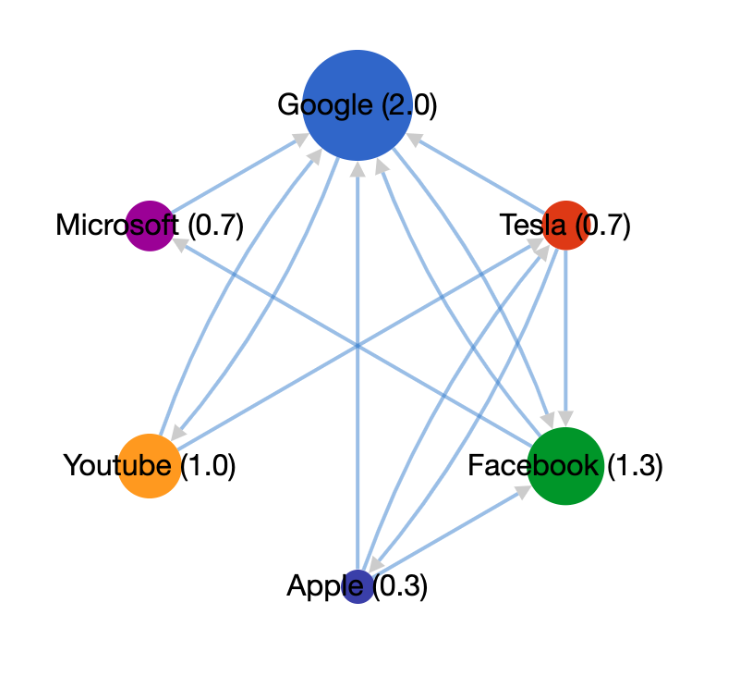
\includegraphics[scale = 0.5]{companies.png}\\
We input this web into our Markov function through a matrix of 1's and 0's. If company i points to company j, we let input$[i][j]$ = 1. Otherwise, input$[i][j]$ = 0. We tell our function which companies correspond to which indices through our companies array.\\
\begin{codeblock}
input = [0 0 1 1 0 0;
         1 0 0 1 0 1; #input[i][j] = true if i goes to j
         1 1 0 0 0 0;
         1 0 0 0 1 0;
         1 0 0 0 0 0;
         1 1 1 0 0 0;]
companies = ["Google", "Tesla", "Youtube", "Facebook", "Microsoft", "Apple"]
\end{codeblock}

\textbf{Populating Our Markov Matrix}\\
We convert our input matrix into a Markov matrix based on our naive random walk implementation. The function takes a company, adds up all the ones into the variable count, and replaces every instance of 1 with the reciprocal of count.\\
\begin{codeblock}
function markov(input, companies)
    m = Array{Float64}(undef, size(input,1), size(input,2))
    for row = 1 : size(input, 1)
        count = 0
        for col = 1 : size(input, 2)
            count = count + input[row, col]
        end
        for col = 1 : size(input, 2)
            if input[row, col] == 1
                m[col, row] = 1/count
            end
        end
    end
\end{codeblock}
\textbf{Applying the Damping Factor}\\
We apply a damping factor to our matrix to ensure it is a regular markov matrix. Like Google's own algorithm, we use a beta of 0.15.
\begin{codeblock}
beta = 0.15
q = 1/size(input,1)
for row = 1 : size(input, 1)
    for col = 1 : size(input, 2)
        m[row, col] = (1-beta)*(m[row, col]) + beta * q
    end
end
\end{codeblock}
\textbf{Taking the Eigenvector}\\
In order to get the steady state vector, we take the eigenvector that corresponds with the eigenvalue that equals 1. We then take the real parts of the eigenvector and normalize it.
\begin{codeblock}
values, vectors = eigen(m)
index = 1
for i = 1 : size(values, 1)
    if abs(values[i] - 1) < 0.00000001
        index = i
    end
end
v2 = vectors[:,index]
v2 = normalize(v2, 1)
v = Array{Float64}(undef, size(v2))
for i = 1 : size(v, 1)
    v[i] = abs(real(v2[i]))
end
\end{codeblock}
\textbf{Printing the Results}\\
Finally, we print out the results. We use the inputted companies array to get the name of the companies. Then, we print out the companies that correspond to the largest terms in the array.
\begin{codeblock}
printed = zeros(Int8, size(v,1))
for i = 1 : size(v, 1)
    largestIndex = 1
    for j = 1 : size(v, 1)
        if ((v[j] > v[largestIndex]) && (printed[j] == 0)) || printed[largestIndex] == 1
            largestIndex = j
        end
    end
    printed[largestIndex] = 1
    print(i)
    print(". ")
    println(companies[largestIndex])
end
return v
\end{codeblock}
\textbf{Our Results}\\
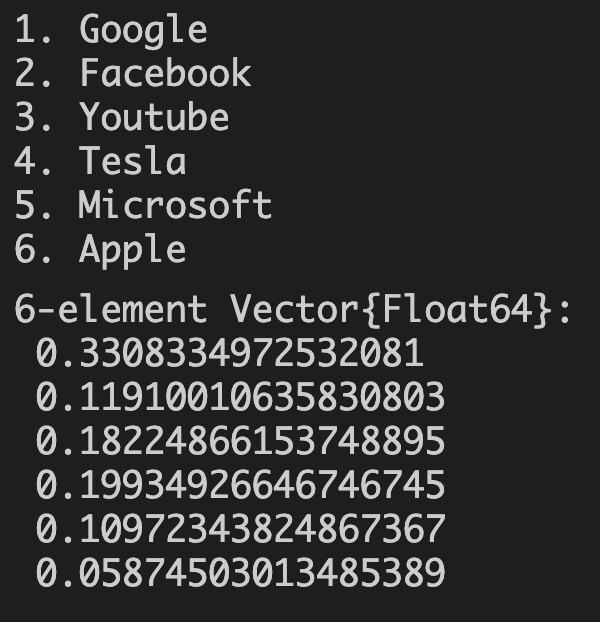
\includegraphics[scale = 0.5]{results.png}\\
We print out the companies that are most relevant from first to last. We also show the steady state vector calculated from our markov matrix. Notice that we had every company point to Google and Google is our highest ranked page.


\section{HITS Algorithm}
Like the PageRank Algorithm, the HITS Algorithm also rates Web pages. It uses the idea of Hubs and Authorities where Hubs hold links to authoritative webpages and Authorities hold link to different hubs. A webpage then receives a high authority score based on how valuable the content of the page is and receives a high hub score if it links to many other high authority scoring pages. \\
\\
The actual algorithm is layed out as follows. The HITS algorithm first generates a root set by gathering the most relevant pages using a search query. It then augments the set into the base set or focused subgraph, which the algorithm is run on, by adding in additional web pages linked to and from the base set.\\
\\
The algorithm then assigns every webpage a hub score and a authority score. So, unlike PageRank where it ranks it on one attribute, HITS uses both an authority and hub score. The authority score is calculated based on how many in-links a page has while the hub score is calculated based on how many out-links a page has. Let x be a $n \: x \:1$ vector holding the authority scores and let y be a $n\: x \: 1$ vector holding the hub scores. We give each page an initial hub and authority score of 1 (initializing x and y to have all 1 entries), and then through every iteration of the algorithm, we adjust the values of each page. Now that we have initialized x and y, the HITS algorithm adjusts these scores with a variation of Kleinberg's original equations when developing the HITS algorithm. It does this until the values in x and y converge and hit a steady state. To think of these vectors in terms of iterations, let $x^k$ be the vector corresponding to the $n \: x\: 1$ vector holding the approximate authority scores at iteration k and let $y^k$ be the vector corresponding to the $n \: x \: 1$ vector holding the approximate hub scores at iteration k. k will continue to increment until $x^k$ and $y^k$ converge. In our case, we will iterate 100 times as an estimate. The following two equations will be used to adjust the scores.

\begin{align*}
    x^k = P^Ty^{k-1}\\
    y^k = Px^k
\end{align*}

Additionally, at each iteration, we need to normalize the vectors $x^k$ and $y^k$. This can be done by dividing the vectors by their magnitudes. After we have performed all 100 iterations, we can then order the pages that correspond with the cols/rows of P by their authority and/or their hub scores.





\section{HITS Code}
\begin{codeblock}
using LinearAlgebra
function HITS(input, companies)
    #HITS ALGORITHM
    y = Array{Float64}(undef, size(input, 1))
    x = Array{Float64}(undef, size(input, 1))
    for i = 1 : size(y, 1)
        y = 1
        x = 1
    end
    for i = 1 : 100
        #COMPUTING X AND Y FOR NEW ITERATION
        x = (transpose(input))*(y)
        y = (input)*(x)
        #NORMALIZING 
        x = normalize(x)
        y = normalize(y)
    end
    
    #CODE CORRECTION
    y2 = Array{Float64}(undef, size(input, 1))
    x2 = Array{Float64}(undef, size(input, 1))
    for row = 1 : size(x, 1)
        x2[row] = x[row, 1]
        y2[row] = y[row, 1]
    end
    y = normalize(y2)
    x = normalize(x2)

    #PRINTING RESULTS
    println("Authority Rankings:")
    printed = zeros(Int8, size(x,1))
    for i = 1 : size(x, 1)
        largestIndex = 1
        for j = 1 : size(x, 1)
            if ((x[j] > x[largestIndex]) && (printed[j] == 0)) || printed[largestIndex] == 1
                largestIndex = j
            end
        end
        printed[largestIndex] = 1
        print(i)
        print(". ")
        println(companies[largestIndex])
    end
    println()
    println("Hub Rankings:")
    printed = zeros(Int8, size(y,1))
    for i = 1 : size(y, 1)
        largestIndex = 1
        for j = 1 : size(y, 1)
            if ((y[j] > y[largestIndex]) && (printed[j] == 0)) || printed[largestIndex] == 1
                largestIndex = j
            end
        end
        printed[largestIndex] = 1
        print(i)
        print(". ")
        println(companies[largestIndex])
    end
    println()
    println("Authority Scores:")
    for i = 1 : size(x, 1)
        println(x[i])
    end
    println()
    println("Hub Scores:")
    for i = 1 : size(y, 1)
        println(y[i])
    end
    println()
    println("Companies Index:")
    for i = 1 : size(companies, 1)
        print(i)
        print(". ")
        println(companies[i])
    end
end
\end{codeblock}
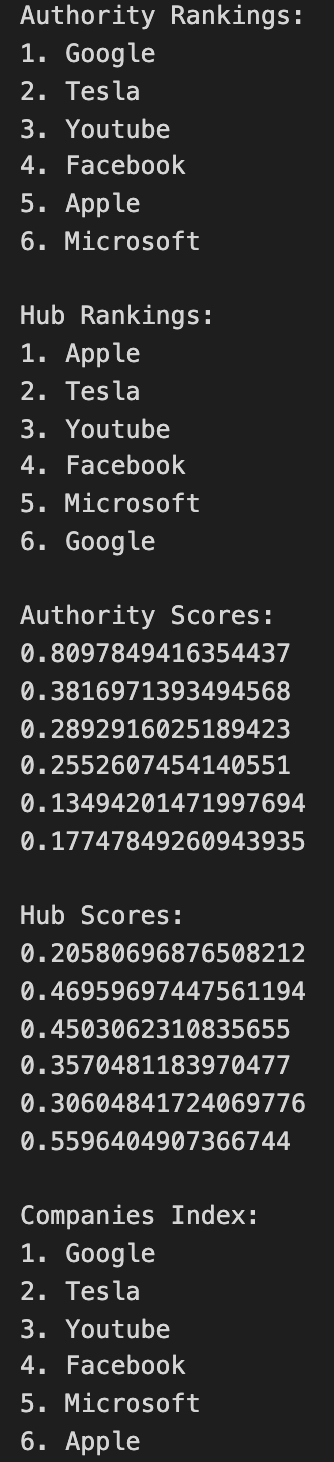
\includegraphics[scale = 0.5]{results2.png}




\begin{thebibliography}{3}
\bibitem{texbook}
Rousseau, Christiane. “How Google Works.” D´Epartement De Math´Ematiques Et De Statistique and CRM Universit´e De Montr´Eal, 5 Aug. 2010. 

\bibitem{textbook}Langville, A. N., &amp; Meyer, C. D. (2012). Google's pagerank and beyond: The science of search engine rankings. Princeton University Press. Retrieved December 3, 2021, from https://gi.cebitec.uni-bielefeld.de/$\_$media/teaching/2019winter/alggr/langville$\_$meyer$\_$2006.pdf. 
\raggedright
\bibitem{textbook}“PageRank.” Wikipedia, Wikimedia Foundation, 2 Dec. 2021, https://en.wikipedia.org/wiki/PageRank. 
\end{thebibliography}
\end{document}
